\documentclass[a4paper, 10pt]{article}%тип документа

%Русский язык
\usepackage[T2A]{fontenc} %кодировка
\usepackage[utf8]{inputenc} %кодировка исходного кода
\usepackage[english,russian]{babel} %локализация и переносы

%отступы 
\usepackage[left=2cm,right=2cm,top=2cm,bottom=3cm,bindingoffset=0cm]{geometry}

%Вставка картинок
\usepackage{graphicx}
\graphicspath{}
\DeclareGraphicsExtensions{.pdf,.png,.jpg, .jpeg}

%Таблицы
\usepackage[table,xcdraw]{xcolor}
\usepackage{booktabs}

%Графики
\usepackage{pgfplots}
\pgfplotsset{compat=1.9}

%Математика
\usepackage{amsmath, amsfonts, amssymb, amsthm, mathtools}

%Заголовок
\author{Нугманов Булат \\ Подлесный Артём \\ группа 827}
\title{Работа 1.4.1 \\ Изучение физического маятника}

\begin{document}
\maketitle
\section*{Цель работы}
Исследовать завсисмость периода колебаний физического маятника от его момента инерции.
\section*{Оборудование}
Физический маятник (однородный стальной стержень), опорная призма,
математический маятник, счетчик числа колебаний, линейка, секундомер.
\section*{Отчёт о работе}
\subsection*{Общая теория}
Физический маятник – любое тело, которое может свободно качаться вокруг вертикальной оси под действием силы тяжести. Движение маятника описывается уравнением:
\begin{equation}
M=I\frac{d^2 \varphi}{dt^2},
\end{equation}
\begin{figure}
\center
\caption{}
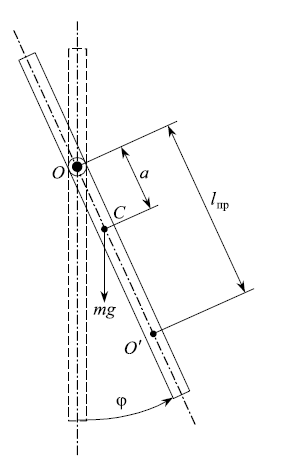
\includegraphics[scale=0.5]{Pic}
\end{figure}

где $I$ –- момент инерции маятника, $ \varphi $ –- угол отклонения маятника от положения равновесия, $t$ –- время, $M$ –- момент сил, действующих на маятник.

На стержне закрепляется опорная призма, острое ребро которой является осью качания маятника.
Призму можно перемещать вдоль ОС, меняя таким образом расстояние от точки опоры маятника до его центра масс.
По теореме Гюйгенса-Штейнера момент инерции маятника: 
\begin{equation}
I =\frac{ml^2}{12}^2+ma^2,
\end{equation}
где $m$ -- масса маятника, $l$ -- длина стержня, $a$ - указано на рисунке.
Момент силы тяжести:
\begin{equation}
M=-mg\sin\varphi\approx-mg\varphi,
\end{equation}
т.к. угол $\varphi$ мал.
Подставляя (2) и (3) в (1), получаем, что 

\begin{equation}
\begin{aligned}
\ddot{\varphi}+\omega^2\varphi=0 \\
\omega^2=\dfrac{ga}{a^2+ \frac{l^2}{12}} \\
\varphi(t)=A\sin(\omega t+\alpha)
\end{aligned}
\end{equation}
Период колебаний равен 
\begin{equation}
T=2\pi=2\pi\sqrt{\dfrac{a^{2}+\dfrac{l^{2}}{12}}{ag}}
\end{equation}
Видно, что период малых колебаний не зависит ни от фазы, ни от амплитуды колебаний. Период колебаний математического маятника определяется формулой
\[T'=2\pi\sqrt{\dfrac{l'}{g}}\]
где l' -- длина математического маятника. Поэтому величину
\begin{equation}
l_{\text{пр}}=a+\dfrac{l^{2}}{12a}
\end{equation}
называют приведенной длиной физического маятника. Тогда исследование зависимости периода колебаний математического маятника заданной длины и физического маятника соответствующей приведенной длины будет хорошим методом проверки теории.
\subsection*{Период при малых колебаниях}
\subsubsection*{Проверка чистоты условий эсперимента}
Однако нетрудно заметить, что полученные выражения выполняются только при малых углах и небольшом моменте сил трения. Для проверки этих предположений, на данной установке проведём эксперимент, зпключающийся в проверке постоянства периода при малы углах и относительно среднем значении a -- 17,5 см. При различных малых углах мы измеряли время совершения 100 колебаний. В данном эксперименте и далее, нажатие на счётчик проиходило в момент, когда маятник проходил положение равновесия. Результаты приведены в таблице 1. Отдельно отметим явно неверные измерения 2-го занчения. Время сильно завышено! Оказалось, что иногда счётчик не всегда срабатывал на нажатие. Однако, в остальном значения отличаются в пределах погрешности, значит при углах $\varphi\leq10^{\circ}$ наши предположения верны.
Стоит так же отметить, что в теоретическом выводе формул не учитывалось, что в точке опоры стержень подвешен с использованием шайбы, которая может влиять на положение центра масс стержня($x_{\text{ц.м.}}$) и его момент инерции($I$), и, как следствие, на длину $l_{\text{пр}}$. Следует проверить, что вклад этой шайбы действительно мал. Для этого посчитаем отношение разности $l_{\text{пр}}$ посчитанной с учетом шайбы, и без, с самой $l_{\text{пр}}$. Вывод формулы для $l'_{\text{пр}}$ достаточно громоздкий, поэтому здесь я выпишу лишь конечную формулу
\begin{equation}
l'_{\text{пр}}=\dfrac{Ml^2+12Ma^2+4mr^2}{12Ma-6mr}
\end{equation}
Здесь $М$ -- масса стрежня, $m$ -- шайбы, $l, r$ -- длины стержня и шайбы соответственно. Данные о них в таблице 3.
%сделай тут эту таблицу, она на стр 3 того эксель файла, который ты мне отправлял по этой лабе.
Таким образом из формулы можно найти $\Delta l_{\text{пр}}$ 
\[\Delta l_{\text{пр}}=l'_{\text{пр}}-l_{\text{пр}}=\dfrac{Ml^2+12Ma^2+4mr^2}{12Ma-6mr}-\dfrac{12a^2+l^2}{12a}\]
Для допустимых значений $a\in [7;40]$ можно найти максимально возможную ошибку для $l_{\text{пр}}$
\begin{equation}
\left(\frac{\Delta l_{\text{пр}}}{l_{\text{пр}}}\right)_{\text{max}}\approx 0,001 
\end{equation}
Эта оценка позволяет утверждать, что влиянием шайбы на $l_{\text{пр}}$ можно принебречь.
\subsubsection*{Проведение эксперимента и обработка полученных результатов}

\begin{table}[]
\caption{}
\center
\begin{tabular}{|
>{\columncolor[HTML]{FFC702}}c |
>{\columncolor[HTML]{FFFFFF}}c |
>{\columncolor[HTML]{FFFFFF}}c |}
\hline
n & \cellcolor[HTML]{FFC702}$\alpha,^{\circ}$ & \cellcolor[HTML]{FFC702}$T_{100}$, c \\ \hline
1 & 10                                         & 162,63                               \\ \hline
2 & 5                                          & 171,25                               \\ \hline
3 & 3                                          & 162,71                               \\ \hline
4 & 5                                          & 162,53                               \\ \hline
\end{tabular}
\end{table}

%пронумеруй таблицы, пожалуйста
На таблице 2 продемонстрированы результаты нашего эксперимента по снятию зависимости периода малых колебаний от расстояния до точки опоры $a$. Для определенного угла мы измеряли время совершения 100 колебаний. В данном эксперименте и далее, нажатие на счётчик проиходило в момент, когда маятник проходил положение равновесия.
Так же были проведены промежуточные измерения, где мы замечали время для 50 колебаний. По полученным данным вычислялся период, и мы сравнивали период за полное число колебаний, и за половину. Как видно из таблицы, эта разница много меньше самого периода, поэтому можно считать, что со временем период почти не изменяется. Отдельно отметим явно неверные измерения занчения для $a=43$, произошло это по той же причине, что и раньше, и в дальнейшем это значение мы перемерили. Из формулы (5) следует
\begin{equation}
aT^2=\frac{4\pi^2}{g}a^2+\dfrac{4\pi^2l^2}{12g}
\end{equation}
\begin{table}[]
\center
\begin{tabular}{|c|c|c|c|c|c|c|c|c|}
\hline
\rowcolor[HTML]{FE0000} 
n  & a, см & N   & $T_{N}$, c & $T_{\text{ср.}}$, c & $N_{1}$ & $T_{N_{1}}$, c & $T_{1\text{ср.}}$, c & $T_{1\text{ср.}}-T_{\text{ср.}}$ \\ \hline
1  & 17,5  & 100 & 162,62     & 1,626               & 50 & -           & -                    & -                                \\ \hline
2  & 47,0  & 100 & 161,50     & 1,615               & 50 & -           & -                    & -                                \\ \hline
3  & 43,0  & 100 & 168,94     & 1,689               & 50 & 89,17       & 1,783                & 0,0940                           \\ \hline
4  & 39,0  & 100 & 156,31     & 1,563               & 50 & 78,00       & 1,560                & -0,0031                          \\ \hline
5  & 35,0  & 100 & 154,00     & 1,540               & 50 & 77,00       & 1,540                & 0,0000                           \\ \hline
6  & 43,0  & 100 & 158,63     & 1,586               & 50 & 79,13       & 1,583                & -0,0037                          \\ \hline
7  & 31,0  & 100 & 153,21     & 1,532               & 50 & 76,00       & 1,520                & -0,0121                          \\ \hline
8  & 27,0  & 100 & 153,00     & 1,530               & 50 & 76,17       & 1,523                & -0,0066                          \\ \hline
9  & 23,0  & 100 & 155,37     & 1,554               & 50 & 77,50       & 1,550                & -0,0037                          \\ \hline
10 & 19,0  & 100 & 160,00     & 1,600               & 50 & 80,10       & 1,602                & 0,0020                           \\ \hline
11 & 15,0  & 50  & 84,85      & 1,697               & 25 & 42,50       & 1,700                & 0,0030                           \\ \hline
12 & 11,0  & 50  & 94,00      & 1,880               & 30 & 57,00       & 1,900                & 0,0200                           \\ \hline
13 & 7,0   & 40  & 91,75      & 2,294               & 34 & 78,00       & 2,294                & 0,0004                           \\ \hline
\end{tabular}
\end{table}
\subsection*{Немалые колебания}
Рассмотрим теперь немалые колебания для этого в уравнении (3) не будем приближать $\sin x\approx x$. Тогда наше уравнеиние будет выглядеть так:
\begin{equation}
\begin{aligned}
\ddot{\varphi}+\omega_{0}^2\sin\varphi=0 \\
\omega_{0}^2=\dfrac{ga}{a^2+ \frac{l^2}{12}}
\end{aligned}
\end{equation}
Естественно, период уже будет зависеть от амплитуды, а в пределе, при малых углах, мы получим период, соответствующий $\omega_{0}$. Решая данный дифур, получаем, что:
\begin{equation}
\begin{aligned}
T=4\sqrt{\frac{l}{g}}K(\sin\frac{\alpha}{2}) \\
K(x)=\int\limits_{0}^{\frac{\pi}{2}}\frac{d\varphi}{\sqrt{1-x^2\sin^2\varphi}}
\end{aligned}
\end{equation}
$K(x)$ - называется полным эллиптичесским интегралом первого рода, а $\alpha$ - амплитуда колебаний. Разлагая полученную специальную функцию по малости аргумента, получаем:
\begin{equation}
\begin{aligned}
T=2\pi\sqrt{\frac{l}{g}}\left(1+\frac{1}{4}\sin^2\frac{\alpha}{2}+\frac{9}{64}\sin^4\frac{\alpha}{2}+\dots\right)
\end{aligned}
\end{equation}
%ЫСЁ!
\begin{figure}
\caption{}
\center
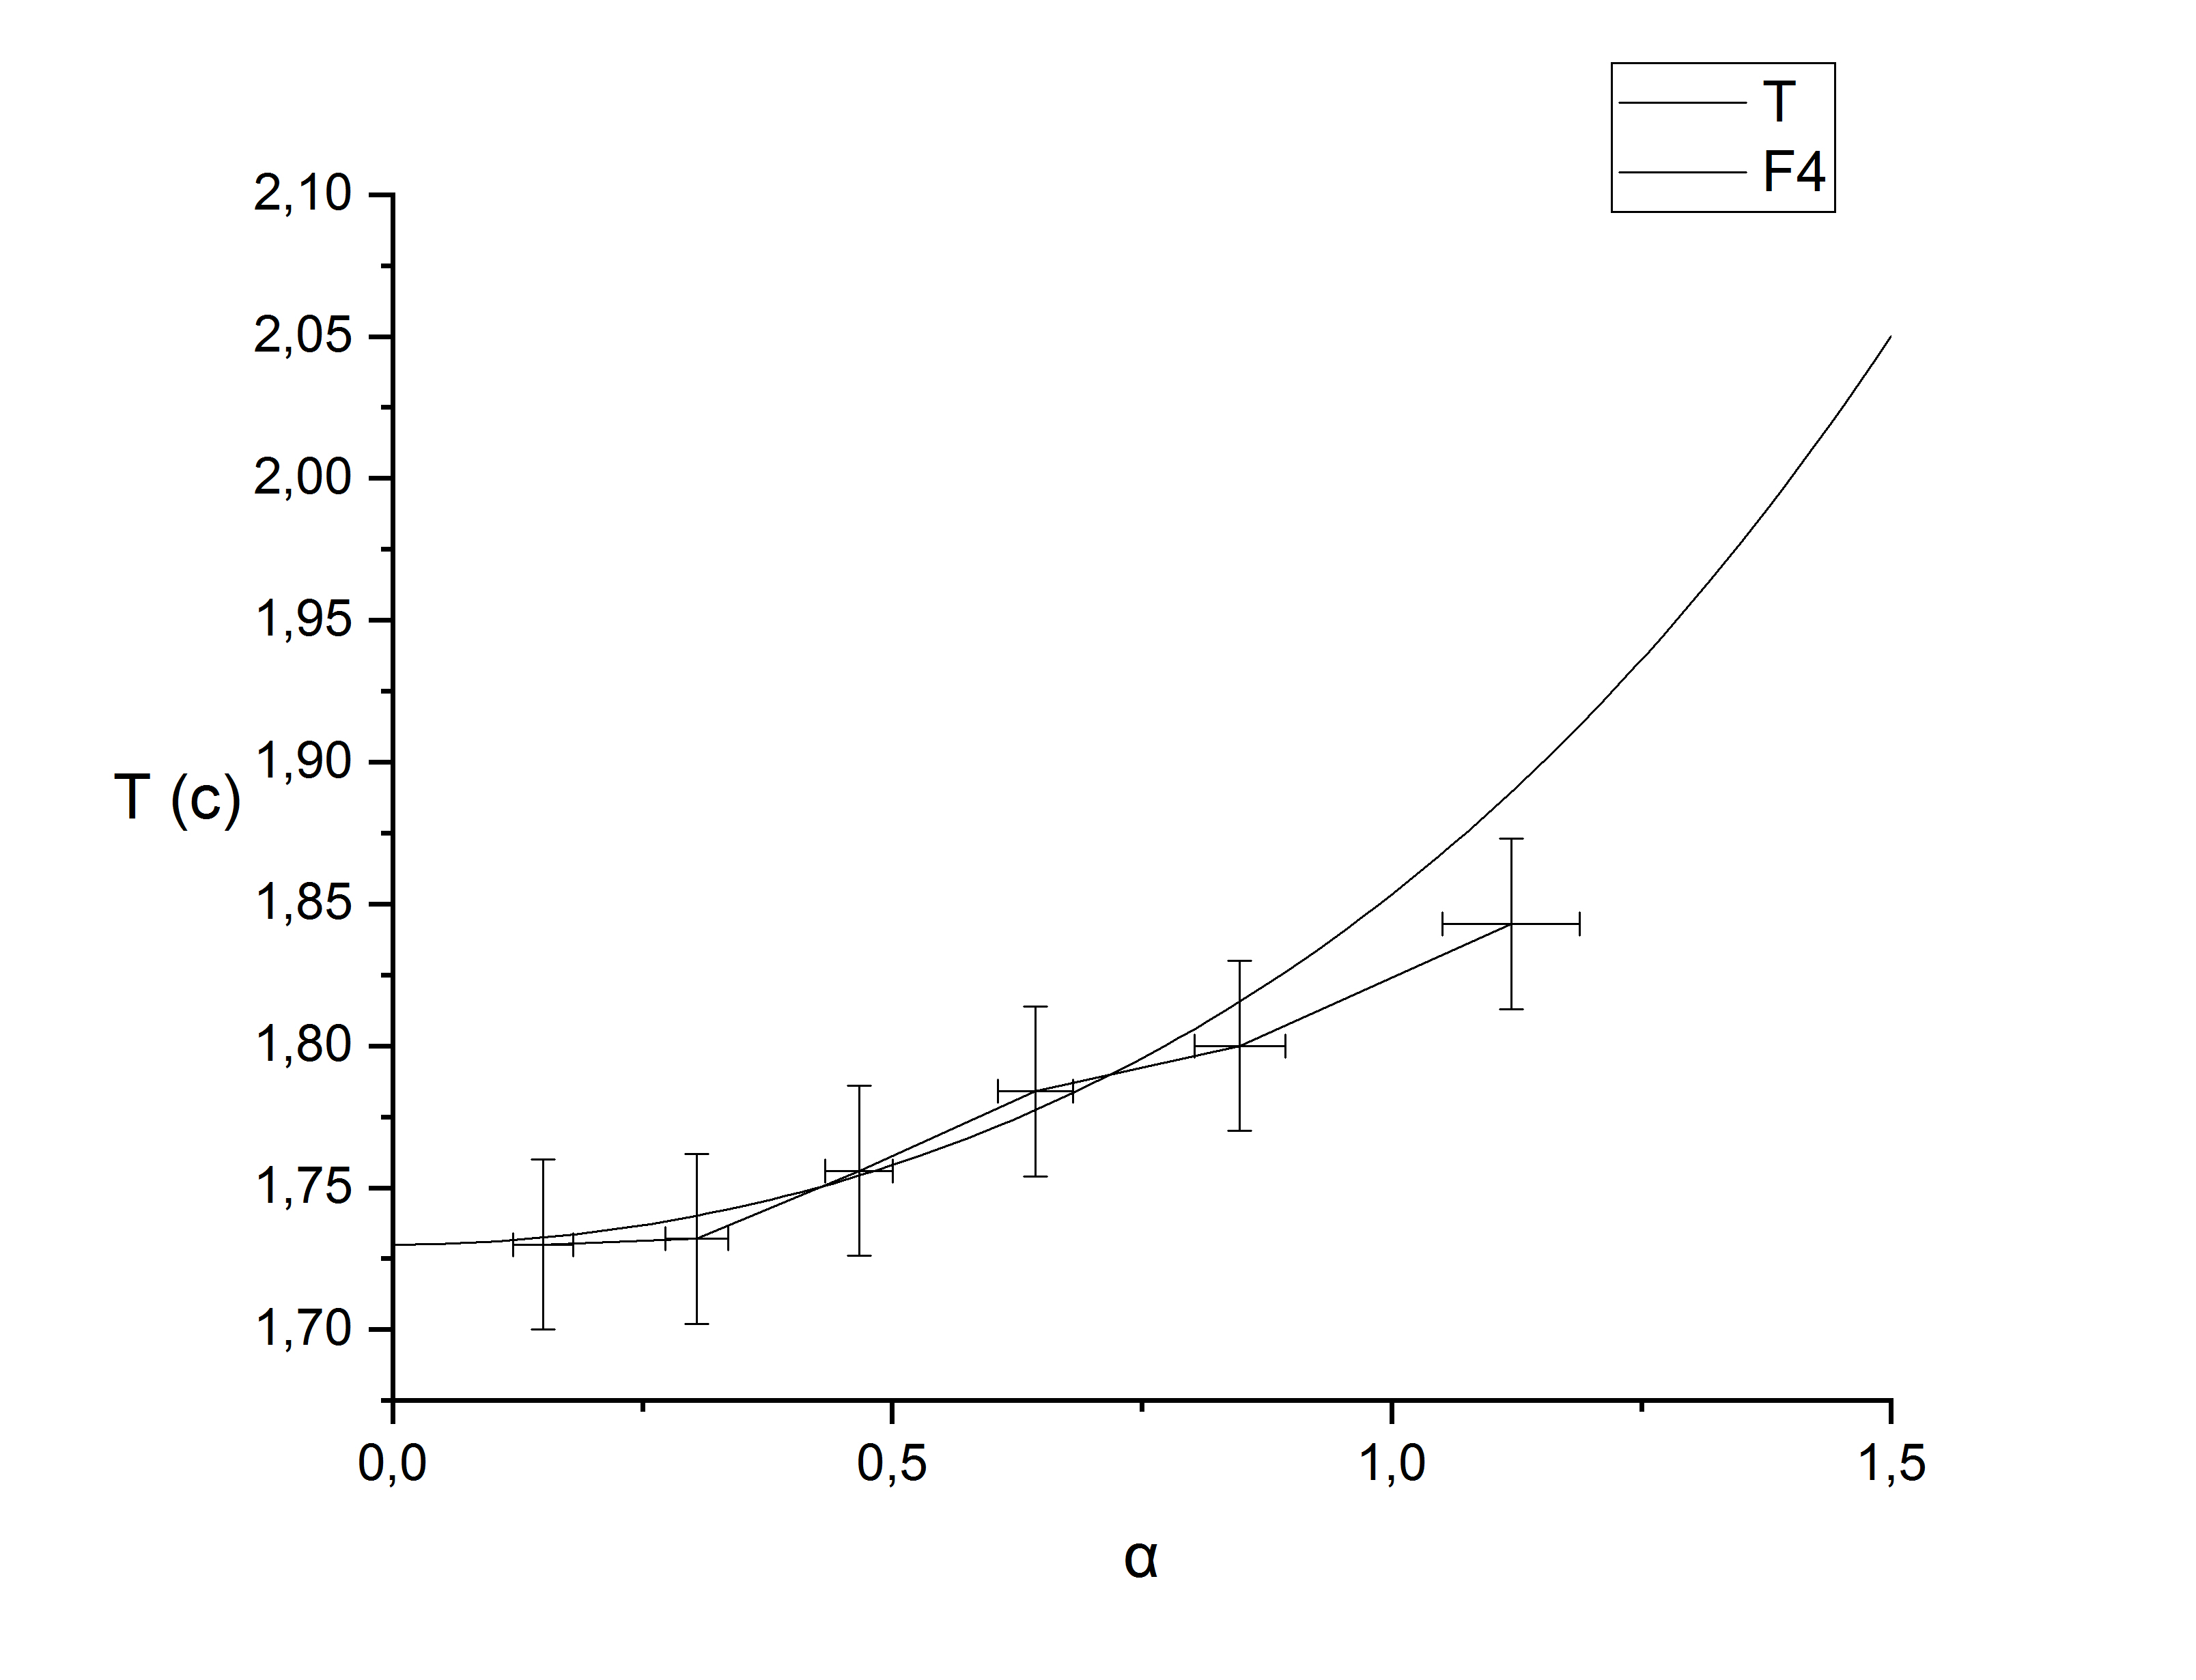
\includegraphics[scale=0.5]{GR1}
\end{figure}
Как видно из  графика, теория непримениима при больших углах. На графике указаны кресты лишь экспериментальных ошибок. А всё потому, что мы сделали допущение об отсутствии трения.
\subsection*{Вязкое трение}
Закон Стокса из теории вязкого трения гласит, что при малых скоростях сила трения, действующая на шарик в среде выражается так:
\begin{equation}
\begin{aligned}
F_{\text{тр.}}=-6\pi rv\mu,
\end{aligned}
\end{equation}
где $r$ -- радиус шарика, $v$ -- скорость шарика, $\mu$ - вязкость.
Для экспериментальной проверки формулы, оценим вязкость воздуха, полученную из данной формулы.
2-ой закон Ньютона будет написан в виде:
\begin{equation}
\begin{aligned}
\ddot{x}-2p\dot{x}+\omega_{0}^2\sin x=0\text{,  где  }
p=\frac{3\pi r\mu}{m}
\end{aligned}
\end{equation}
В ходе решения для малых колебаний выражение для амплитуды:
\begin{equation}
\begin{aligned}
A=Ae^{-pt}
\end{aligned}
\end{equation}
Получается, самый простой метод оценить p -- построить график $-ln(A)$ от t, что мы и сделаем. ("y" в таблице означает проекцию шарика на горизонтальную ось)
\begin{table}[h]
\centering
\caption{}
\label{my-label}
\begin{tabular}{|c|c|c|}
\hline
\rowcolor[HTML]{9B9B9B} 
y, см & $\alpha$ & Т, с  \\ \hline
40    & 0,643501 & 565   \\ \hline
30    & 0,466765 & 329   \\ \hline
20    & 0,304693 & 243   \\ \hline
10    & 0,150568 & 108   \\ \hline
50    & 18       & 1,8   \\ \hline
60    & 18,43    & 1,843 \\ \hline
\end{tabular}
\end{table}
\begin{figure}
\center
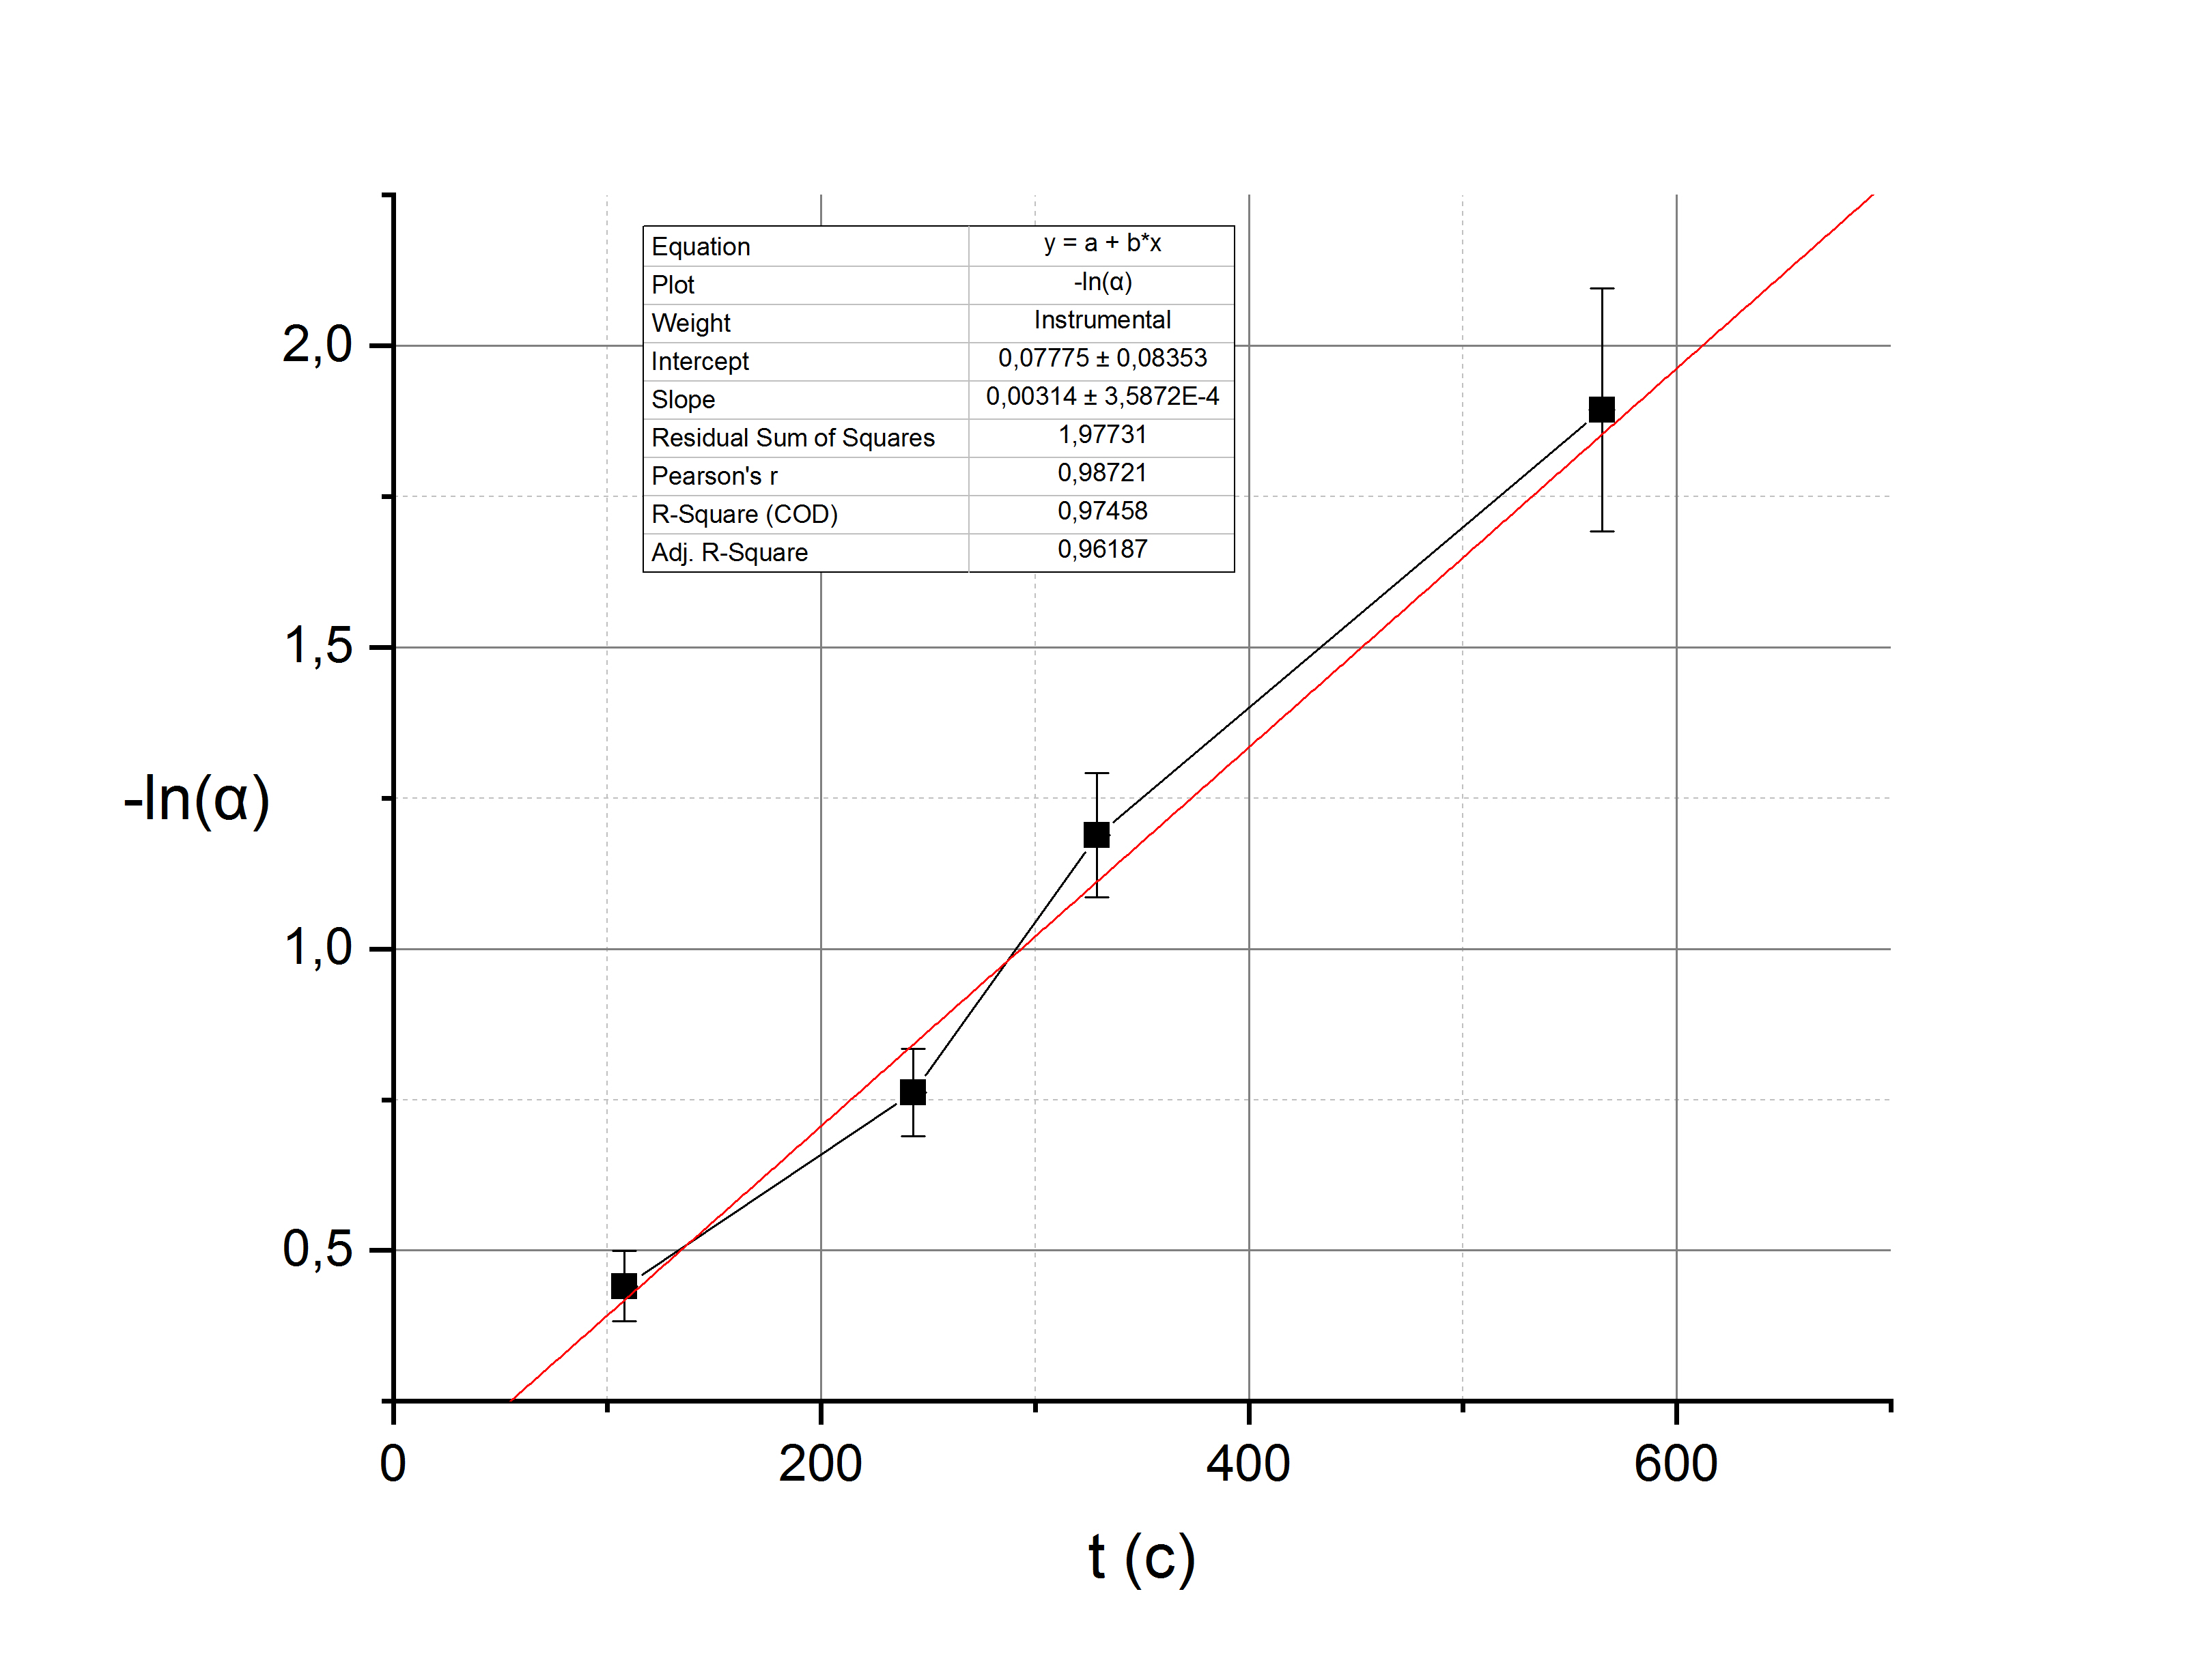
\includegraphics[scale=0.5]{GR3}
\end{figure}
p из графика по МНК получается $(3.14\pm0.36)\text{c}^{-1}$, что соответсвтует $\mu=13,2$ мПа$\cdot$c (m=100 г, r=2.52 см).
%Всё!

Однако, полученное значение, на сильно расходиться от указанного в таблице (18,6 мкПа$\cdot$с). Понятно, что мы использовали теорию малых колебаний там, где она неприменима, но расхождение относительно синуса не очень велико. По крайней мере это не должно давать расхождение на 3 порядка. Самое время задуматься о применимости нашей формулы, то есть о малости скорости. Оносительным безразмерным показателем "малости" является число Рейнольдса.
Выражение для числа Рейнольдса:
\begin{equation}
\begin{aligned}
Re=\frac{\rho_{\text{среды}} vd}{\mu}
\end{aligned}
\end{equation}
$d$ -- здесь некоторый параметр, характеризующий размеры движущегося тела. Мы возьмём его равным диаметру шарика. Вязкость воздуха возьмём из таблицы, считая что температура воздуха близка к 27$^{\circ}$С. Скорость шарика вставим как половину амплитудного значения. Полученное число Рейнольдса $\sim$ 2800 ($\mu$ = 18,6 мкПа$\cdot$ с, $\rho$ = 1,18 кг/м$^3$, v = 1,8 м/с), что никак нельзя считать малым значением. (Для данного случая малым может быть значение порядка 1 или меньше.)

Этим объясняется неприменимость написанных выше формул. 

\section*{Вывод}
Таким образом, мы изучили зависимость периода физического маятника от его параметров: положения центра масс, момента инерции. Также мы убедились, что период при малых колебаниях почти не зависит от амплитуды.%Артём, напиши сюда, что считаешь нужным по той части работы, которую делал.

Также мы измерили зависимость между периодом и амплитудой в модели немалых колебаний. В пределах применимости, теоретическая кривая хорошо фитингует полученные точки, хотя и заявлять о полном подтверждении теории тоже нельзя -- погрешность слишком большая. Однако уменьшить её в данном методе было трудно. Погрешность времени можно уменьшить лишь увеличив количество колебаний, но это при этом нельзя пренебрегать трением, а теория немалых колебаний нами не разработана. Погршешность в определении угла вносила простая неточность нашей системы. Угол мерился  при помощи определения проекции колеблющегося маятника на горизонтальную ось! Очевидно, установка не подходит для проведениия подобного эксперимента. 

И хотя мы использовали кривые руки и установку, мы отметили, что затухание колебаний по экспоненте с натяжкой (прямая еле касается границ погрешностей точек), но может быть применима. Однако причина этого точно не в наличии вязкого трения, ведь оно формируется при ламинарных, то есть устоявшихся, течениях воздуха, а число Рейнольдса в эксперименте очень велико. В подтверждение этому говорит в тысячу раз расходящееся с табличным значение вязкости воздуха.
\end{document}
